% Options for packages loaded elsewhere
\PassOptionsToPackage{unicode}{hyperref}
\PassOptionsToPackage{hyphens}{url}
\PassOptionsToPackage{dvipsnames,svgnames,x11names}{xcolor}
%
\documentclass[
  11pt,
]{article}

\usepackage{amsmath,amssymb}
\usepackage{iftex}
\ifPDFTeX
  \usepackage[T1]{fontenc}
  \usepackage[utf8]{inputenc}
  \usepackage{textcomp} % provide euro and other symbols
\else % if luatex or xetex
  \usepackage{unicode-math}
  \defaultfontfeatures{Scale=MatchLowercase}
  \defaultfontfeatures[\rmfamily]{Ligatures=TeX,Scale=1}
\fi
\usepackage{lmodern}
\ifPDFTeX\else  
    % xetex/luatex font selection
\fi
% Use upquote if available, for straight quotes in verbatim environments
\IfFileExists{upquote.sty}{\usepackage{upquote}}{}
\IfFileExists{microtype.sty}{% use microtype if available
  \usepackage[]{microtype}
  \UseMicrotypeSet[protrusion]{basicmath} % disable protrusion for tt fonts
}{}
\makeatletter
\@ifundefined{KOMAClassName}{% if non-KOMA class
  \IfFileExists{parskip.sty}{%
    \usepackage{parskip}
  }{% else
    \setlength{\parindent}{0pt}
    \setlength{\parskip}{6pt plus 2pt minus 1pt}}
}{% if KOMA class
  \KOMAoptions{parskip=half}}
\makeatother
\usepackage{xcolor}
\usepackage[margin=0.75in]{geometry}
\setlength{\emergencystretch}{3em} % prevent overfull lines
\setcounter{secnumdepth}{-\maxdimen} % remove section numbering
% Make \paragraph and \subparagraph free-standing
\ifx\paragraph\undefined\else
  \let\oldparagraph\paragraph
  \renewcommand{\paragraph}[1]{\oldparagraph{#1}\mbox{}}
\fi
\ifx\subparagraph\undefined\else
  \let\oldsubparagraph\subparagraph
  \renewcommand{\subparagraph}[1]{\oldsubparagraph{#1}\mbox{}}
\fi

\usepackage{color}
\usepackage{fancyvrb}
\newcommand{\VerbBar}{|}
\newcommand{\VERB}{\Verb[commandchars=\\\{\}]}
\DefineVerbatimEnvironment{Highlighting}{Verbatim}{commandchars=\\\{\}}
% Add ',fontsize=\small' for more characters per line
\usepackage{framed}
\definecolor{shadecolor}{RGB}{241,243,245}
\newenvironment{Shaded}{\begin{snugshade}}{\end{snugshade}}
\newcommand{\AlertTok}[1]{\textcolor[rgb]{0.68,0.00,0.00}{#1}}
\newcommand{\AnnotationTok}[1]{\textcolor[rgb]{0.37,0.37,0.37}{#1}}
\newcommand{\AttributeTok}[1]{\textcolor[rgb]{0.40,0.45,0.13}{#1}}
\newcommand{\BaseNTok}[1]{\textcolor[rgb]{0.68,0.00,0.00}{#1}}
\newcommand{\BuiltInTok}[1]{\textcolor[rgb]{0.00,0.23,0.31}{#1}}
\newcommand{\CharTok}[1]{\textcolor[rgb]{0.13,0.47,0.30}{#1}}
\newcommand{\CommentTok}[1]{\textcolor[rgb]{0.37,0.37,0.37}{#1}}
\newcommand{\CommentVarTok}[1]{\textcolor[rgb]{0.37,0.37,0.37}{\textit{#1}}}
\newcommand{\ConstantTok}[1]{\textcolor[rgb]{0.56,0.35,0.01}{#1}}
\newcommand{\ControlFlowTok}[1]{\textcolor[rgb]{0.00,0.23,0.31}{#1}}
\newcommand{\DataTypeTok}[1]{\textcolor[rgb]{0.68,0.00,0.00}{#1}}
\newcommand{\DecValTok}[1]{\textcolor[rgb]{0.68,0.00,0.00}{#1}}
\newcommand{\DocumentationTok}[1]{\textcolor[rgb]{0.37,0.37,0.37}{\textit{#1}}}
\newcommand{\ErrorTok}[1]{\textcolor[rgb]{0.68,0.00,0.00}{#1}}
\newcommand{\ExtensionTok}[1]{\textcolor[rgb]{0.00,0.23,0.31}{#1}}
\newcommand{\FloatTok}[1]{\textcolor[rgb]{0.68,0.00,0.00}{#1}}
\newcommand{\FunctionTok}[1]{\textcolor[rgb]{0.28,0.35,0.67}{#1}}
\newcommand{\ImportTok}[1]{\textcolor[rgb]{0.00,0.46,0.62}{#1}}
\newcommand{\InformationTok}[1]{\textcolor[rgb]{0.37,0.37,0.37}{#1}}
\newcommand{\KeywordTok}[1]{\textcolor[rgb]{0.00,0.23,0.31}{#1}}
\newcommand{\NormalTok}[1]{\textcolor[rgb]{0.00,0.23,0.31}{#1}}
\newcommand{\OperatorTok}[1]{\textcolor[rgb]{0.37,0.37,0.37}{#1}}
\newcommand{\OtherTok}[1]{\textcolor[rgb]{0.00,0.23,0.31}{#1}}
\newcommand{\PreprocessorTok}[1]{\textcolor[rgb]{0.68,0.00,0.00}{#1}}
\newcommand{\RegionMarkerTok}[1]{\textcolor[rgb]{0.00,0.23,0.31}{#1}}
\newcommand{\SpecialCharTok}[1]{\textcolor[rgb]{0.37,0.37,0.37}{#1}}
\newcommand{\SpecialStringTok}[1]{\textcolor[rgb]{0.13,0.47,0.30}{#1}}
\newcommand{\StringTok}[1]{\textcolor[rgb]{0.13,0.47,0.30}{#1}}
\newcommand{\VariableTok}[1]{\textcolor[rgb]{0.07,0.07,0.07}{#1}}
\newcommand{\VerbatimStringTok}[1]{\textcolor[rgb]{0.13,0.47,0.30}{#1}}
\newcommand{\WarningTok}[1]{\textcolor[rgb]{0.37,0.37,0.37}{\textit{#1}}}

\providecommand{\tightlist}{%
  \setlength{\itemsep}{0pt}\setlength{\parskip}{0pt}}\usepackage{longtable,booktabs,array}
\usepackage{calc} % for calculating minipage widths
% Correct order of tables after \paragraph or \subparagraph
\usepackage{etoolbox}
\makeatletter
\patchcmd\longtable{\par}{\if@noskipsec\mbox{}\fi\par}{}{}
\makeatother
% Allow footnotes in longtable head/foot
\IfFileExists{footnotehyper.sty}{\usepackage{footnotehyper}}{\usepackage{footnote}}
\makesavenoteenv{longtable}
\usepackage{graphicx}
\makeatletter
\def\maxwidth{\ifdim\Gin@nat@width>\linewidth\linewidth\else\Gin@nat@width\fi}
\def\maxheight{\ifdim\Gin@nat@height>\textheight\textheight\else\Gin@nat@height\fi}
\makeatother
% Scale images if necessary, so that they will not overflow the page
% margins by default, and it is still possible to overwrite the defaults
% using explicit options in \includegraphics[width, height, ...]{}
\setkeys{Gin}{width=\maxwidth,height=\maxheight,keepaspectratio}
% Set default figure placement to htbp
\makeatletter
\def\fps@figure{htbp}
\makeatother

\usepackage{fvextra}
\DefineVerbatimEnvironment{Highlighting}{Verbatim}{breaklines,commandchars=\\\{\}}
\DefineVerbatimEnvironment{OutputCode}{Verbatim}{breaklines,commandchars=\\\{\}}
\fvset{breaksymbolleft={}, breakindent=1em}
\makeatletter
\@ifpackageloaded{caption}{}{\usepackage{caption}}
\AtBeginDocument{%
\ifdefined\contentsname
  \renewcommand*\contentsname{Table of contents}
\else
  \newcommand\contentsname{Table of contents}
\fi
\ifdefined\listfigurename
  \renewcommand*\listfigurename{List of Figures}
\else
  \newcommand\listfigurename{List of Figures}
\fi
\ifdefined\listtablename
  \renewcommand*\listtablename{List of Tables}
\else
  \newcommand\listtablename{List of Tables}
\fi
\ifdefined\figurename
  \renewcommand*\figurename{Figure}
\else
  \newcommand\figurename{Figure}
\fi
\ifdefined\tablename
  \renewcommand*\tablename{Table}
\else
  \newcommand\tablename{Table}
\fi
}
\@ifpackageloaded{float}{}{\usepackage{float}}
\floatstyle{ruled}
\@ifundefined{c@chapter}{\newfloat{codelisting}{h}{lop}}{\newfloat{codelisting}{h}{lop}[chapter]}
\floatname{codelisting}{Listing}
\newcommand*\listoflistings{\listof{codelisting}{List of Listings}}
\makeatother
\makeatletter
\makeatother
\makeatletter
\@ifpackageloaded{caption}{}{\usepackage{caption}}
\@ifpackageloaded{subcaption}{}{\usepackage{subcaption}}
\makeatother
\ifLuaTeX
  \usepackage{selnolig}  % disable illegal ligatures
\fi
\usepackage{bookmark}

\IfFileExists{xurl.sty}{\usepackage{xurl}}{} % add URL line breaks if available
\urlstyle{same} % disable monospaced font for URLs
\hypersetup{
  pdftitle={Homework 4},
  pdfauthor={Nick Climaco},
  colorlinks=true,
  linkcolor={blue},
  filecolor={Maroon},
  citecolor={Blue},
  urlcolor={Blue},
  pdfcreator={LaTeX via pandoc}}

\title{Homework 4}
\author{Nick Climaco}
\date{February 24, 2024}

\begin{document}
\maketitle

\renewcommand*\contentsname{Table of contents}
{
\hypersetup{linkcolor=}
\setcounter{tocdepth}{3}
\tableofcontents
}
\section{KJ Chapter 3: Data
Preprocessing}\label{kj-chapter-3-data-preprocessing}

\subsection{Exercise 1}\label{exercise-1}

The UC Irvine Machine Learning Repository6 contains a data set related
to glass identification. The data consist of 214 glass samples labeled
as one of seven class categories. There are nine predictors, including
the refractive index and percentages of eight elements: Na, Mg, Al, Si,
K, Ca, Ba, and Fe. The data can be accessed via:

\begin{Shaded}
\begin{Highlighting}[]
\NormalTok{kaggle.api.authenticate()}
\NormalTok{kaggle.api.dataset\_download\_files(}\StringTok{\textquotesingle{}uciml/glass\textquotesingle{}}\NormalTok{, path}\OperatorTok{=}\StringTok{\textquotesingle{}./\textquotesingle{}}\NormalTok{, unzip}\OperatorTok{=}\VariableTok{True}\NormalTok{)}
\end{Highlighting}
\end{Shaded}

\begin{Shaded}
\begin{Highlighting}[]
\NormalTok{df\_glass }\OperatorTok{=}\NormalTok{ pd.read\_csv(}\StringTok{\textquotesingle{}glass.csv\textquotesingle{}}\NormalTok{)}

\NormalTok{df\_glass}
\end{Highlighting}
\end{Shaded}

\begin{longtable}[]{@{}lllllllllll@{}}
\toprule\noalign{}
& RI & Na & Mg & Al & Si & K & Ca & Ba & Fe & Type \\
\midrule\noalign{}
\endhead
\bottomrule\noalign{}
\endlastfoot
0 & 1.52101 & 13.64 & 4.49 & 1.10 & 71.78 & 0.06 & 8.75 & 0.00 & 0.0 &
1 \\
1 & 1.51761 & 13.89 & 3.60 & 1.36 & 72.73 & 0.48 & 7.83 & 0.00 & 0.0 &
1 \\
2 & 1.51618 & 13.53 & 3.55 & 1.54 & 72.99 & 0.39 & 7.78 & 0.00 & 0.0 &
1 \\
3 & 1.51766 & 13.21 & 3.69 & 1.29 & 72.61 & 0.57 & 8.22 & 0.00 & 0.0 &
1 \\
4 & 1.51742 & 13.27 & 3.62 & 1.24 & 73.08 & 0.55 & 8.07 & 0.00 & 0.0 &
1 \\
... & ... & ... & ... & ... & ... & ... & ... & ... & ... & ... \\
209 & 1.51623 & 14.14 & 0.00 & 2.88 & 72.61 & 0.08 & 9.18 & 1.06 & 0.0 &
7 \\
210 & 1.51685 & 14.92 & 0.00 & 1.99 & 73.06 & 0.00 & 8.40 & 1.59 & 0.0 &
7 \\
211 & 1.52065 & 14.36 & 0.00 & 2.02 & 73.42 & 0.00 & 8.44 & 1.64 & 0.0 &
7 \\
212 & 1.51651 & 14.38 & 0.00 & 1.94 & 73.61 & 0.00 & 8.48 & 1.57 & 0.0 &
7 \\
213 & 1.51711 & 14.23 & 0.00 & 2.08 & 73.36 & 0.00 & 8.62 & 1.67 & 0.0 &
7 \\
\end{longtable}

\begin{Shaded}
\begin{Highlighting}[]
\NormalTok{X }\OperatorTok{=}\NormalTok{ df\_glass.drop([}\StringTok{\textquotesingle{}Type\textquotesingle{}}\NormalTok{], axis }\OperatorTok{=} \DecValTok{1}\NormalTok{)}
\NormalTok{y }\OperatorTok{=}\NormalTok{ df\_glass.Type}
\end{Highlighting}
\end{Shaded}

\subsubsection{Part A}\label{part-a}

\paragraph{Using visualizations, explore the predictor variables to
understand their distributions as well as the relationships between
predictors.}\label{using-visualizations-explore-the-predictor-variables-to-understand-their-distributions-as-well-as-the-relationships-between-predictors.}

\begin{Shaded}
\begin{Highlighting}[]
\CommentTok{\# calc corr between predictors}
\NormalTok{correlation\_matrix }\OperatorTok{=}\NormalTok{ X.corr()}
\NormalTok{mask }\OperatorTok{=}\NormalTok{ np.triu(correlation\_matrix) }\CommentTok{\# halves the matrix }
\NormalTok{np.fill\_diagonal(mask, }\VariableTok{False}\NormalTok{) }\CommentTok{\# shows the diagonal }
\NormalTok{sns.heatmap(correlation\_matrix, cmap }\OperatorTok{=} \StringTok{\textquotesingle{}coolwarm\textquotesingle{}}\NormalTok{, annot}\OperatorTok{=}\VariableTok{True}\NormalTok{, mask }\OperatorTok{=}\NormalTok{ mask ).set\_title(}\StringTok{\textquotesingle{}Correlation Matrix for Glass Data\textquotesingle{}}\NormalTok{)}
\NormalTok{plt.show()}
\end{Highlighting}
\end{Shaded}

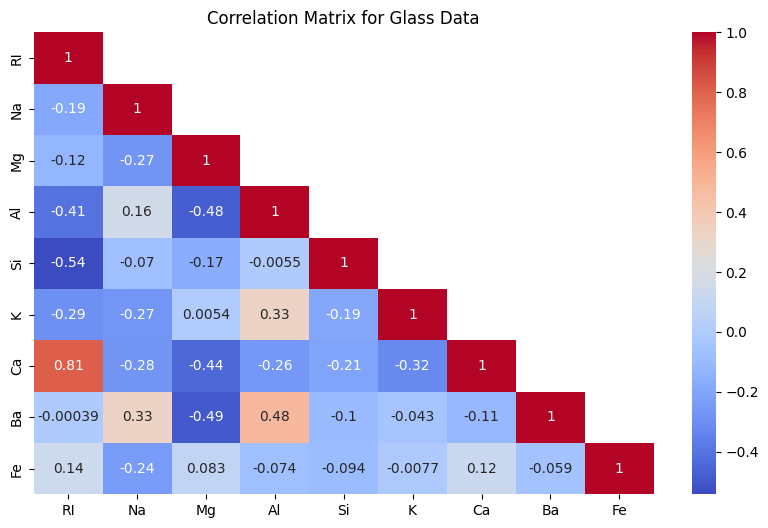
\includegraphics{hw4_files/figure-pdf/cell-7-output-1.png}

\begin{Shaded}
\begin{Highlighting}[]
\NormalTok{df\_glass.describe().T }\CommentTok{\# transpose it since its easier to view this way}
\end{Highlighting}
\end{Shaded}

\begin{longtable}[]{@{}lllllllll@{}}
\toprule\noalign{}
& count & mean & std & min & 25\% & 50\% & 75\% & max \\
\midrule\noalign{}
\endhead
\bottomrule\noalign{}
\endlastfoot
RI & 214.0 & 1.518365 & 0.003037 & 1.51115 & 1.516522 & 1.51768 &
1.519157 & 1.53393 \\
Na & 214.0 & 13.407850 & 0.816604 & 10.73000 & 12.907500 & 13.30000 &
13.825000 & 17.38000 \\
Mg & 214.0 & 2.684533 & 1.442408 & 0.00000 & 2.115000 & 3.48000 &
3.600000 & 4.49000 \\
Al & 214.0 & 1.444907 & 0.499270 & 0.29000 & 1.190000 & 1.36000 &
1.630000 & 3.50000 \\
Si & 214.0 & 72.650935 & 0.774546 & 69.81000 & 72.280000 & 72.79000 &
73.087500 & 75.41000 \\
K & 214.0 & 0.497056 & 0.652192 & 0.00000 & 0.122500 & 0.55500 &
0.610000 & 6.21000 \\
Ca & 214.0 & 8.956963 & 1.423153 & 5.43000 & 8.240000 & 8.60000 &
9.172500 & 16.19000 \\
Ba & 214.0 & 0.175047 & 0.497219 & 0.00000 & 0.000000 & 0.00000 &
0.000000 & 3.15000 \\
Fe & 214.0 & 0.057009 & 0.097439 & 0.00000 & 0.000000 & 0.00000 &
0.100000 & 0.51000 \\
Type & 214.0 & 2.780374 & 2.103739 & 1.00000 & 1.000000 & 2.00000 &
3.000000 & 7.00000 \\
\end{longtable}

\begin{Shaded}
\begin{Highlighting}[]
\NormalTok{X.hist(grid}\OperatorTok{=}\VariableTok{False}\NormalTok{)}
\NormalTok{plt.tight\_layout()}
\NormalTok{plt.show()}
\end{Highlighting}
\end{Shaded}

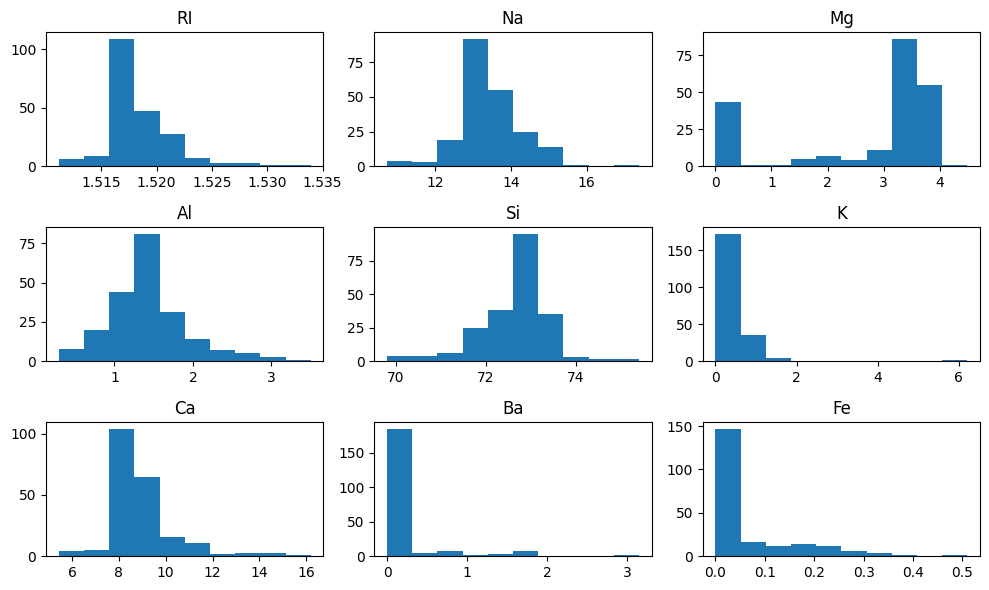
\includegraphics{hw4_files/figure-pdf/cell-9-output-1.png}

\begin{Shaded}
\begin{Highlighting}[]
\NormalTok{fig, ax }\OperatorTok{=}\NormalTok{ plt.subplots(nrows}\OperatorTok{=}\DecValTok{3}\NormalTok{, ncols}\OperatorTok{=}\DecValTok{3}\NormalTok{)}

\ControlFlowTok{for}\NormalTok{ i, col }\KeywordTok{in} \BuiltInTok{enumerate}\NormalTok{(X.columns):}
\NormalTok{     sns.boxplot(x}\OperatorTok{=}\NormalTok{col, data}\OperatorTok{=}\NormalTok{X, ax}\OperatorTok{=}\NormalTok{ax.flatten()[i])}

\NormalTok{fig.suptitle(}\StringTok{\textquotesingle{}Boxplot for each Predictor\textquotesingle{}}\NormalTok{)}
\NormalTok{plt.tight\_layout()}
\NormalTok{plt.show()   }
\end{Highlighting}
\end{Shaded}

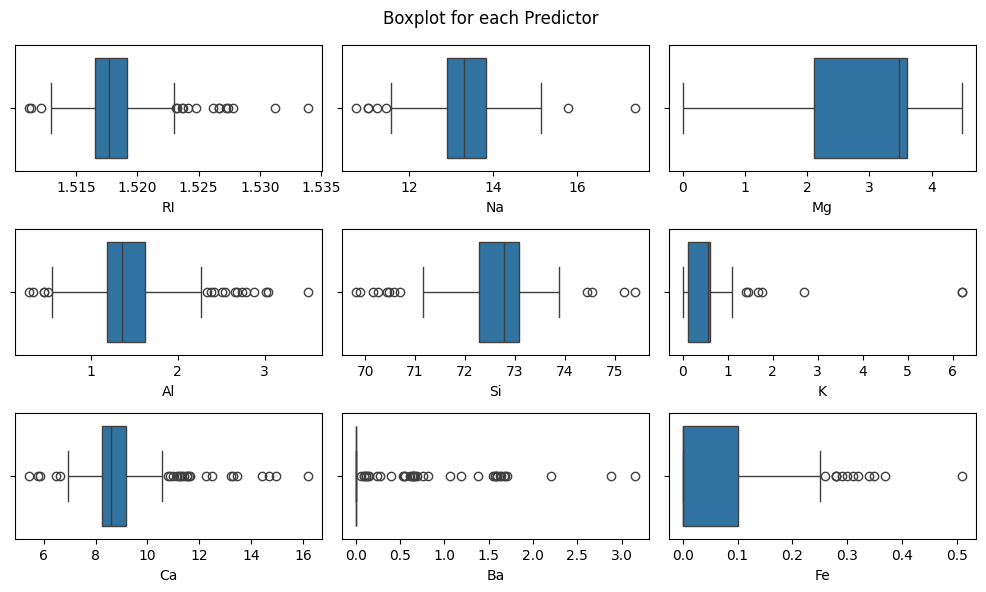
\includegraphics{hw4_files/figure-pdf/cell-10-output-1.png}

\subsubsection{Part B}\label{part-b}

\paragraph{Do there appear to be any outliers in the data? Are any
predictors
skewed?}\label{do-there-appear-to-be-any-outliers-in-the-data-are-any-predictors-skewed}

If we consider data outside the IQR, then almost all predictors have
outliers with the expection of \texttt{Mg} column having no visuable
outliers. The column with the most outliers seems to be \texttt{Ba}
suggests that Barium is not a common ingredient in glass while the
amount of magnesiumn found in glass fairly common. Moreover, another
method to detect outliers that I like to use is z-scores where we
consider a datapoint to be an outliers if it is more than 1.96 standard
deviations away from the mean since that should capture 95\% of the
data.

All of the predictors are skewed albeit some are more skewed than
others. For instance, \texttt{K},\texttt{Ba} and \texttt{Fe} looks more
like a poisson distribution with a low-value lambda.

\subsubsection{Part C}\label{part-c}

\paragraph{Are there any relevant transformations of one or more
predictors that might improve the classification
model?}\label{are-there-any-relevant-transformations-of-one-or-more-predictors-that-might-improve-the-classification-model}

Some transformations we might use to improve the classification model is
a log transform so that the distribution resembles normality.
Specifically for models that assume normal data such as a linear
regression. Another transformation, I would suggest is to standardize
the predictors where their scales are from -1 to 1 or normalize the
scale from 0-1 which ever works better for the task.

\begin{center}\rule{0.5\linewidth}{0.5pt}\end{center}

\subsection{Exercise 2}\label{exercise-2}

The soybean data can also be found at the UC Irvine Machine Learning
Repository. Data were collected to predict disease in 683 soybeans. The
35 predictors are mostly categorical and include information on the
environmental conditions (e.g., temperature, precipitation) and plant
conditions (e.g., left spots, mold growth). The outcome labels consist
of 19 distinct classes.

\begin{Shaded}
\begin{Highlighting}[]
\ImportTok{from}\NormalTok{ ucimlrepo }\ImportTok{import}\NormalTok{ fetch\_ucirepo }
  
\NormalTok{soybean\_large }\OperatorTok{=}\NormalTok{ fetch\_ucirepo(}\BuiltInTok{id}\OperatorTok{=}\DecValTok{90}\NormalTok{) }
  
\NormalTok{X }\OperatorTok{=}\NormalTok{ soybean\_large.data.features }
\NormalTok{y }\OperatorTok{=}\NormalTok{ soybean\_large.data.targets }
\end{Highlighting}
\end{Shaded}

\begin{Shaded}
\begin{Highlighting}[]
\NormalTok{X.head()}
\end{Highlighting}
\end{Shaded}

\begin{longtable}[]{@{}llllllllllll@{}}
\toprule\noalign{}
& date & plant-stand & precip & temp & hail & ... & mold-growth &
seed-discolor & seed-size & shriveling & roots \\
\midrule\noalign{}
\endhead
\bottomrule\noalign{}
\endlastfoot
0 & 6.0 & 0.0 & 2.0 & 1.0 & 0.0 & ... & 0.0 & 0.0 & 0.0 & 0.0 & 0.0 \\
1 & 4.0 & 0.0 & 2.0 & 1.0 & 0.0 & ... & 0.0 & 0.0 & 0.0 & 0.0 & 0.0 \\
2 & 3.0 & 0.0 & 2.0 & 1.0 & 0.0 & ... & 0.0 & 0.0 & 0.0 & 0.0 & 0.0 \\
3 & 3.0 & 0.0 & 2.0 & 1.0 & 0.0 & ... & 0.0 & 0.0 & 0.0 & 0.0 & 0.0 \\
4 & 6.0 & 0.0 & 2.0 & 1.0 & 0.0 & ... & 0.0 & 0.0 & 0.0 & 0.0 & 0.0 \\
\end{longtable}

\begin{Shaded}
\begin{Highlighting}[]
\NormalTok{X.shape}
\end{Highlighting}
\end{Shaded}

\begin{verbatim}
(307, 35)
\end{verbatim}

\begin{Shaded}
\begin{Highlighting}[]
\NormalTok{y.nunique()}
\end{Highlighting}
\end{Shaded}

\begin{verbatim}
class    19
dtype: int64
\end{verbatim}

Making sure the correct dataset is loaded. It seems the data from UC
Irvine has less observations from the data in the R library mlbench

\subsubsection{Part A}\label{part-a-1}

\paragraph{Investigate the frequency distributions for the categorical
predictors. Are any of the distributions degenerate in the ways
discussed earlier in this
chapter?}\label{investigate-the-frequency-distributions-for-the-categorical-predictors.-are-any-of-the-distributions-degenerate-in-the-ways-discussed-earlier-in-this-chapter}

\begin{Shaded}
\begin{Highlighting}[]
\NormalTok{X.hist(grid}\OperatorTok{=}\VariableTok{False}\NormalTok{)}
\NormalTok{plt.tight\_layout()}
\NormalTok{plt.show()}
\end{Highlighting}
\end{Shaded}

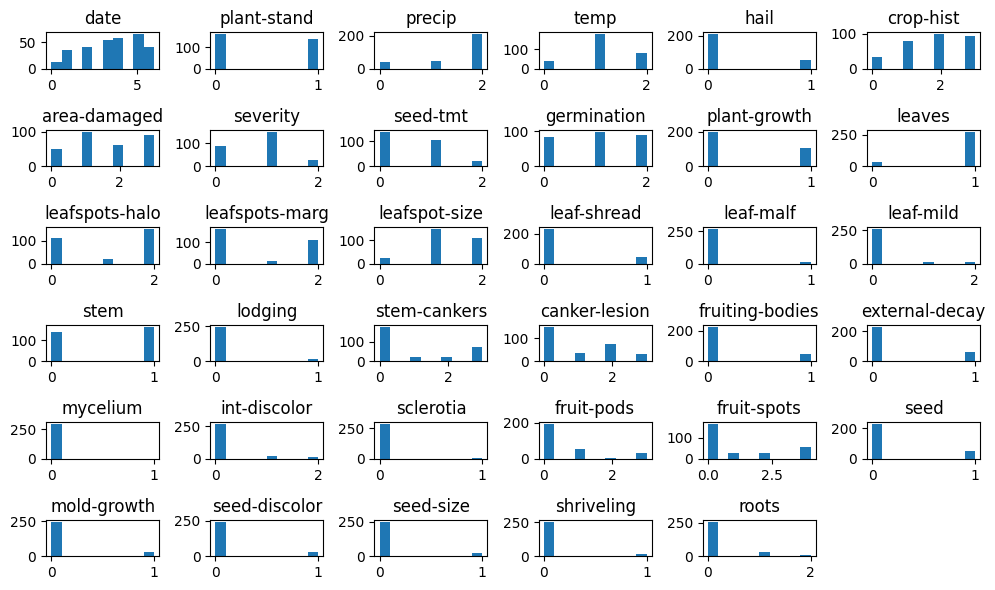
\includegraphics{hw4_files/figure-pdf/cell-15-output-1.png}

\begin{Shaded}
\begin{Highlighting}[]
\NormalTok{X.mycelium.value\_counts()}
\end{Highlighting}
\end{Shaded}

\begin{verbatim}
mycelium
0.0    294
1.0      2
Name: count, dtype: int64
\end{verbatim}

\begin{Shaded}
\begin{Highlighting}[]
\NormalTok{X.mycelium.var()}
\end{Highlighting}
\end{Shaded}

\begin{verbatim}
0.006733852496564359
\end{verbatim}

While there no predictors will a 100\% denegerate distribution, there
are definitely a lot of predictors that are very close to the denegerate
distribution just to name a few: \texttt{mycelium} is the closest to a
complete degenerate distribution, and others like \texttt{seed-size},
\texttt{shriveling}, and \texttt{sclerotia}.

\subsubsection{Part B}\label{part-b-1}

\paragraph{Roughly 18\% of the data are missing. Are there particular
predictors that are more likely to be missing? Is the pattern of missing
data related to the
classes?}\label{roughly-18-of-the-data-are-missing.-are-there-particular-predictors-that-are-more-likely-to-be-missing-is-the-pattern-of-missing-data-related-to-the-classes}

\begin{Shaded}
\begin{Highlighting}[]
\NormalTok{X.isna().}\BuiltInTok{sum}\NormalTok{().sort\_values(ascending}\OperatorTok{=}\VariableTok{False}\NormalTok{).head(}\DecValTok{10}\NormalTok{)}
\end{Highlighting}
\end{Shaded}

\begin{verbatim}
hail               41
lodging            41
severity           41
seed-tmt           41
germination        36
fruit-spots        35
fruiting-bodies    35
shriveling         35
seed-discolor      35
leaf-mild          30
dtype: int64
\end{verbatim}

We have 41 rows with at least one missing data.

\begin{Shaded}
\begin{Highlighting}[]
\DecValTok{41} \OperatorTok{/}\NormalTok{ X.shape[}\DecValTok{0}\NormalTok{]}
\end{Highlighting}
\end{Shaded}

\begin{verbatim}
0.13355048859934854
\end{verbatim}

\begin{Shaded}
\begin{Highlighting}[]
\NormalTok{df\_soybean.mycelium.isna().}\BuiltInTok{sum}\NormalTok{()}
\end{Highlighting}
\end{Shaded}

\begin{verbatim}
11
\end{verbatim}

\begin{Shaded}
\begin{Highlighting}[]
\NormalTok{df\_soybean.groupby(}\StringTok{\textquotesingle{}class\textquotesingle{}}\NormalTok{).}\BuiltInTok{apply}\NormalTok{(}\KeywordTok{lambda}\NormalTok{ x: x.isna().}\BuiltInTok{sum}\NormalTok{().}\BuiltInTok{sum}\NormalTok{()).sort\_values(ascending }\OperatorTok{=} \VariableTok{False}\NormalTok{)}
\end{Highlighting}
\end{Shaded}

\begin{verbatim}
class
phytophthora-rot               390
cyst-nematode                  144
herbicide-injury                80
diaporthe-pod-&-stem-blight     68
2-4-d-injury                    30
brown-spot                       0
brown-stem-rot                   0
charcoal-rot                     0
bacterial-pustule                0
alternarialeaf-spot              0
diaporthe-stem-canker            0
downy-mildew                     0
frog-eye-leaf-spot               0
bacterial-blight                 0
phyllosticta-leaf-spot           0
anthracnose                      0
powdery-mildew                   0
purple-seed-stain                0
rhizoctonia-root-rot             0
dtype: int64
\end{verbatim}

This exercise reiterates the importance of domain knowledge in this
field. For the soybean dataset, understanding the ``mycelium'' is a
fungi, after a google search, represents whether the soybean plant has
fungi or not clarifies the possible reasons why it is missing 11 values.
Due to the nature of this binary condition indicates that those 11 was
possibly not recorded as the cause of missingness. The documentation
confirms that all predictors are categorical with ranks ranging from
2-6.

Futher examiniation of the data reveals that certain soybean classes
hold higher concentration of missing data suggesting systematic
missingness rather missingness completely at random (MCAR). Leading our
examination to the data colleciton process for specifically those
classes.

\subsubsection{Part C}\label{part-c-1}

\paragraph{Develop a strategy for handling missing data, either by
eliminating predictors or
imputation.}\label{develop-a-strategy-for-handling-missing-data-either-by-eliminating-predictors-or-imputation.}

We would consider completely removing the 2-3 classes with the most
missing values because we suspect that the missing value was possibly
due to errors in data collection. While for rest of the missing values,
we suggest employing a combination of imputation techniques in a way it
mitigates its impact on the ditribution of each predictor and the
quality of the predictions after model training.



\end{document}
